\documentclass[11pt, oneside]{article}   	% use "amsart" instead of "article" for AMSLaTeX format
\usepackage{geometry}                		% See geometry.pdf to learn the layout options. There are lots.
\geometry{letterpaper}                   		% ... or a4paper or a5paper or ... 
%\geometry{landscape}                		% Activate for for rotated page geometry
%\usepackage[parfill]{parskip}    		% Activate to begin paragraphs with an empty line rather than an indent
\usepackage{graphicx}				% Use pdf, png, jpg, or eps§ with pdflatex; use eps in DVI mode
								% TeX will automatically convert eps --> pdf in pdflatex		
\usepackage{amssymb}
\usepackage{amsmath}
\usepackage{setspace}
\usepackage[square,sort,comma,numbers]{natbib} \bibpunct{(}{)}{;}{author-year}{}{,} 
\usepackage[hidelinks]{hyperref}


\title{Local PCA Shows How Population Structure Differs Along the Genome}
\author{Han Li, Peter Ralph}
%\date{}							% Activate to display a given date or no date

\usepackage{color}
\newcommand{\plr}[1]{{\em \color{blue} #1}}


\begin{document}
\maketitle
%\section{}
%\subsection{}
\doublespacing

\plr{Note: your intro focuses on PCA more than mine, which is trying to be about population structure generally.}

\section{Introduction}

The kinship matrix contains the kinship coefficient for pairwise individuals. 
Kinship coefficient defines the genetic relatedness between individuals.
It is the probability that two alleles randomly selected from two individuals are inherited from the most recent common ancester.
It could be estimated from given pedigree or from genome-wide covariances of genotype markers. 
It is well-known that for kinship matrix, actual relatednesses have a lot of noise about the expected value, and depend on where on the genome you look; this is why scans for selective sweeps work.
Populations are often structured in some way while there are systematic genetic variation between populations. 

About 37 years ago, \citet{menozzi1978synthetic} first applied principal component analysis (PCA) in population genetics to construct maps summarizing genetic variation \citep{menozzi1978synthetic}. 
Nowadays, PCA is a widely used powerful non-parametric method to extract information from genetic data.  
PCA results are derived from the covariance matrix of genotype matrix. 
The results of PCA can be directly related to the underlying genealogical history of the samples, 
such as coalescence time (time to most recent common ancestor) and migration rate between populations \citep{novembre2008interpreting,mcvean2009genealogical}. 
Through dimension-reduction, PCA can identify key components of population structure, which describes how different samples are related, and are often closely related to geography. 
Plots of the first two principal components (PCs) can mimic the samples' geographic origin to some extent. 
Since population structure describes how different samples are related, samples living closer tend to be more genetically similar and thus tend to be clustered in PC plots \citep{novembre2008genes,patterson2006population}. 
However this relatedness is limited while there's recent migration or for group with nongeographic kinship patterns,for example, social or religious groups. \citep{astle2009population}

PCA is often used in genome-wide association studies (GWAS) for stratification correction \citep{price2006principal}. 
However, different parts of genome have different genetic features. 
First, each site of DNA may have different gene tree. 
The covariance matrix of genotype matrix averages those gene trees. 
For a genomic region, if individuals have alleles closer in gene tree, they tends to be more close in PC projections for that region. 
Different DNA segments may have different gene tree and therefore different population structure for those segments. 
Second, the strength of linked selection differs for different DNA segments, and produces different population structure in region under linked selection compared to other region. 
Selective sweeps cause local recent ancestry or short trees.
Balancing selection causes deep trees.
Background selection causes shallow ones.
Third, if a chromosome inversion is polymorphic in the sample, the regions around the breakpoints of inversions usually have high linkage disequilibrium and the two directions of a inversion will have different linked alleles around the breakpoints. Recombination suppression across inversions thus results in different genome structure and population structure. 
Other effects, like noise, introgression might also influence population structure.

Investigating the genomic variation along the genome can help us to have a
better understanding of the relation between genome structure and population
structure, and could possibly lead to more powerful methods for GWAS.

To investigate this, we cut each chromosome into windows (with hundreds to
thousands of SNPs in each), applied PCA to each window, and visualized how
population structure, as summarized by PCA, varies along windows.

In this project, we used SNP data for human, \textit{Medicago truncatula}, and
whole genome sequencing data for \textit{Drosophila}.  Based on the principal
components, we can estimate the similarity of population structure contained in
each genome window.  To quantify similarity of population structure between
windows, we constructed for each window an approximate, scaled covariance
matrix based on the first two PCs measured the pairwise Euclidean distance
between those matrices.  We use multidimensional scaling to visualize the
relationships between windows, which reduces the pairwise distance matrix to
lower dimension while preserving the distance information between windows as
well as possible \citep{borg2005modern}.  To interpret the results of MDS, we
combine known genome feature information for each species, such as the
distribution of inversions, and heterochromatin and gene density along the
genome. Each species showed distinct patterns, reflecting differences in their
biology. 

Other methods for visualizing population structure are like STRUCTURE,
\citep{pritchard2000inference,falush2003inference,
falush2007inference,hubisz2009inferring} 
model-based approach,
\citep{yang2012modelbased} 
maps of heterozygosity
\citep{ramachandran2005support}. 

A number of methods for dimensionality reduction also use a strategy of ``local PCA''
\citep[e.g.][]{manjon2013diffusion,kambhatla1997dimension,weingessel2000local,roweis2000nonlinear},
performing PCA not on the entire dataset but instead on subsets,
providing ``local'' pictures which are then stitched back together to give a global picture.
Our method shares this common thread, but differs somewhat in the context and goals,
and future methods may benefit from this substantial literature \citep[reviewed in][]{vandermaaten2009dimensionality}.


\section{Other Introduction}

Catchy start: the kinship matrix goes back to almost Mendel and is essential in GWAS;
however, it is well-known that actual relatednesses have a lot of noise about the expected value,
and depend on where on the genome you look;
this is why scans for selective sweeps work.

Review of kinship matrix: 
it's either an expected kinship, given the pedigree;
or an estimated genome-wide average.
Wright's path coefficients \citep{wright1943isolation}.
Why it helps with confounding for GWAS.
Graham \& Vince's paper, maybe.
Like IBD, is only well-defined in a known pedigree, up to the founders.
Kinship and confounding reviewed in \citet{astle2009population}.

Kinship matrices differ for sex chromosomes and the like.

Review of selection causing differential patterns along the genome.
Locally everything is treelike (gene trees);
kinship matrix is an average of these (write equation for this).
Selective sweeps cause local recent ancestry/short trees.
Balancing selection causes deep trees.
Background selection, shallow ones.
Extreme examples of free gene flow in some places between species: e.g. Heliconius.
Introgression may be nonuniform, e.g. neanderthal, others.
Refs: hitchhiking \citep{maynardsmith1974hitchhiking},
\citet{kim2011hitchhiking} study hitchhiking in a spatially subdivided population,
\citet{mcvean2007structure} looks at the effect of selection on LD.
\citet{barton2000genetic} reviews hitchhiking.
\citet{bierne2010distinctive} discusses how hitchhiking effect decreases with geographic distance.
\citet{charlesworth2003review} reviews patterns of diversity, relating spatial structure to effects of selection.

Review of methods looking along the genome:
argweaver, HMM between species, ???

What is "population structure"?
Asks which "populations" are closely related, more diverged, how much diversity do they harbor.
Often geographic.
Vital in exploratory data analysis.
It is a summary of kinship: 
lack of migration between pops causes a deficit in connections through the pedigree,
and so affects kinship.
Wright defined $F_{ST}$ in \citep{wright1949genetical}, and says ``It has probably occurred to the reader that the coefficientof inbreeding may mean very different
things in different cases.''

Review of methods for visualizing pop structure:
PCA, structure \citep{falush2003inference}, EEMS, \citep{petkova2014visualizing}, \citep{yang2012modelbased},
Maps of heterozygosity \citep{ramachandran2005support}.
Genealogical interpretation of PCA by \citet{mcvean2009genealogical}.
Other semi-related stuff:
estimation of covariance matrices;
local pca(?);



\section{Methods}

\plr{How about: first describe the method; then afterwards, present the three datasets.}

\subsection{Recode the DNA sequence to a matrix consisting of 0,1,2 (and NA).}

\plr{Separate paragraphs for each dataset. Say how many sites, what kind of data, etcetera.}

For human, we use SNP chip data from POPRES \citet{nelson2008population}. There are 3965 samples in total, (346 African-Americas; 73 Asians; 3187 Europeans; 359 Indian Asians), and the 22 autosomes together have 447267 SNPs in this dataset. 
We use the allele that has highest frequency in the samples as the reference allele for each position. 
If an allele is same with the reference allele, we recode it as 0; if an allele is different from the reference allele, we recode it as 1; for positions that have missing data, we recode them as NA. 
Since human genome is diploid, we add the value for the two alleles and then one chromosome will eventually be recode to a sequence consisting of 0,1,2 (and NA).
Then the genome data for human is recoded to a matrix that has 3965 columns, each column for an individual's genotype. 
We process the data separately for the 22 autosomes in human.

For \textit{Drosophila}, we use the sequencing data from DPGP and John pool's lab \citet{lack2015drosophila}, which together has 380 samples from 16 countries.
We first process the sequencing data (from DPGP and John pool's lab) to SNP data by eliminating the positions that have all the same alleles. 
Each chromosome arms we investigated (Chr2L, Chr2R, Chr3L, Chr3R, ChrX) has 2-3 million SNPs.
Due to high density of missing data for some parts in the genome, we then delete the samples with more than 8\% NAs and positions with more than 20\%. 
The cutoff points 8\% and 20\% are determined from the corresponding distributions of NAs in samples and at positions. 
After we got the SNP data for \textit{Drosophila}, we recode it \textit{Drosophila}to matrices with 0,1,2 (and NA) for each chromosome arms (Chr2L, Chr2R, Chr3L, Chr3R, ChrX) similar to the process for human genome. 
Since the \textit{Drosophila} samples here are all homogenous, the matrices are indeed consisting of 0,1 (and NA). 

For \textit{Medicago truncatula}, we use the SNP data from Medicago Hapmap. It has 263 samples from 24 countries. 
We recode it to matrices with 0,1,2 (and NA) for each of the 8 chromosomes. Each chromosome has 3-5 million SNPs

\subsection{PCA in genomic windows}

\plr{this describes PCA, not cutting into windows? and, the next section?}
We cut each recoded matrix into sub matrixes by that have the same columns but fewer rows than the original matrix. Then apply Principal Component Analysis (PCA) on each window. Here's a brief summary about how is PCA carried out on genomic data \citep{mcvean2009genealogical}. Starting with the recoded genotype matrix Z, where Z is a L*N matrix ( L is SNP number ; N is sample size), then zero-center the matrix Z to X to make the data rows have equal mean. ($X_{si}=Z_{si}-\frac{1}{n}\sum_{j=1}^{n}Z_{sj}$) Get the covariance matrix of X (denote as matrix C) and compute the eigenvectors and eigenvalues of the covariance matrix C. ($C=\frac{1}{n-1}XX^{T}$ ) The \textit{i}th principal component is the \textit{i}th eigenvector of C.
\plr{(put equations into the text in the right place)}

PCA on each window is getting the eigenvectors of covariance matrix of the cut recoded matrix. PCA plots generally use PC2 against PC1.
PC1 and PC2 refer to the first and second principal component respectively. 
PCA plots can show population structure, which describes how different samples are related. 
We want to investigate the variation of population structure along the genome. 
So we apply PCA on each window to check the population structure along the genome.
\subsubsection{Choose window length}
The window length should neither be too long or too short. The longer the windows, the more accurate is the estimate of population structure in that window. However, for better resolution, we need to find a length that is reasonably short. If we use the first principal component as a measure of population structure, then to choose a proper length for a
window, we need to find a balance between variance of the first principal components inside a window and that between windows. The variance between windows is estimated as mean variance of the first principal component for each window. The variance inside a window is estimated using the jackknife block when cutting the window into 10 equal size smaller windows \cite{efron1982jackknife}. Table \ref{tab:window_sizes} shows the comparison of variance within a window and that between windows for chromosome arms in \textit{Drosophila}. Finally, we choose 100 SNPs, 1000 SNPs and 10000 SNPs as window length for human, \textit{Drosophila}, and \textit{Medicago} separately.



\begin{table}[ht]
\centering
\begin{tabular}{rllrrrrr}
  \hline
 & chr\_name & win\_length(in SNPs) & 100 & 500 & 10\verb|^|3 & 10\verb|^|4 & 10\verb|^|5 \\ 
  \hline
1 & Chr2L & SE\verb|^|2(within) & 2.05e-03 & 1.64e-03 & 1.18e-03 & 1.68e-04 & 4.02e-05 \\ 
  2 & Chr2L & Var(between) & 2.76e-03 & 2.69e-03 & 2.23e-03 & 6.74e-04 & 3.12e-04 \\ 
  3 & Chr2R & SE\verb|^|2(within) & 2.18e-03 & 1.92e-03 & 1.63e-03 & 5.76e-04 & 1.35e-04 \\ 
  4 & Chr2R & Var(between) & 2.78e-03 & 2.70e-03 & 2.65e-03 & 2.31e-03 & 1.82e-03 \\ 
  5 & Chr3L & SE\verb|^|2(within) & 2.08e-03 & 2.00e-03 & 1.64e-03 & 7.32e-04 & 2.45e-04 \\ 
  6 & Chr3L & Var(between) & 2.60e-03 & 2.52e-03 & 2.40e-03 & 1.68e-03 & 1.89e-03 \\ 
  7 & Chr3R & SE\verb|^|2(within) & 1.95e-03 & 1.76e-03 & 1.44e-03 & 5.87e-04 & 2.03e-04 \\ 
  8 & Chr3R & Var(between) & 2.58e-03 & 2.51e-03 & 2.44e-03 & 1.96e-03 & 1.40e-03 \\ 
  9 & ChrX & SE\verb|^|2(within) & 2.48e-03 & 2.04e-03 & 1.54e-03 & 1.62e-03 & 1.68e-04 \\ 
  10 & ChrX & Var(between) & 2.61e-03 & 2.43e-03 & 2.30e-03 & 3.24e-04 & 1.14e-03 \\ 
   \hline
\end{tabular}
\caption{
Comparison of variance within a window and that between windows for chromosome arms in \textit{Drosophila}.
} \label{tab:window_sizes}
\end{table}

\subsubsection{Similarity of population structure between windows}
We use the first two principal components (PCs) and the corresponding eigenvalues from PCA, and construct a new matrix with the two PCs for each window to stand for the population structure information. 
For example, the constructed matrixes for ith and jth window are as following. 
($\lambda _{1i}$ and $\lambda _{2i}$ are the eigenvalues for the first two PCs for \textit{i}th window; $\lambda _{1j}$ and $\lambda _{2j}$ are the eigenvalues for the first two PCs for \textit{j}th window.) $M_i$ and $M_j$ are the constructed new matrix for \textit{i}th window and \textit{j}th window.
\plr{
Say what $M_i$ and $M_j$ are in the text.  
Also, how about we write $V$ instead of $PC$?  I like to use only one letter for variables, so it's clear it's just one thing, not the product of $P$ and $C$.
And, isn't it $\sqrt{\lambda_{1j}^2+\lambda_{2j}^2}$ on the bottom? Check in the R code (pc{\textunderscore}dist.R).
}

\begin{align}
    M_{i} &= \frac{\lambda_{1i}PC1_{i}PC1_{i}^{T}+\lambda_{2i}PC2_{i}PC2_{i}^{T}}{\lambda_{1i}+\lambda_{2i}} \\
    M_{j} &= \frac{\lambda_{1j}PC1_{j}PC1_{j}^{T}+\lambda_{2j}PC2_{j}PC2_{j}^{T}}{\lambda_{1j}+\lambda_{2j}}
\end{align}

The Euclidean distance $D_{ij}$ between the constructed matrices $M_i$ and $M_j$ stands for the similarity of population structure for the \textit{i}th window and \textit{j}th window. 
Due to the property of eigenvectors,we could use the following method to calculate the pairwise distance greatly saving time and space.

\plr{Define $D$.}

\begin{equation}
    \begin{aligned}
        V_{1}&=\sqrt{\frac{\lambda _{1i}}{\lambda _{1i}+\lambda _{2i}}}PC1_{i} \qquad
        V_{2}&=\sqrt{\frac{\lambda _{2i}}{\lambda _{1i}+\lambda _{2i}}}PC2_{i} \\
        U_{1}&=\sqrt{\frac{\lambda _{1j}}{\lambda _{1j}+\lambda _{2j}}}PC1_{j} \qquad
        U_{2}&=\sqrt{\frac{\lambda _{2j}}{\lambda _{1j}+\lambda _{2j}}}PC2_{j}
    \end{aligned}
\end{equation}

\begin{align}
    \begin{split}
    D_{ij} &= 
        \left \{
                \left ( 
                    V_{1}\cdot V_{1}^{} 
                \right )^{2}
                + \left ( V_{2}\cdot V_{2}^{} \right )^{2}
                + \left ( U_{1}\cdot U_{1}^{} \right )^{2} 
                +\left ( U_{2}\cdot U_{2}^{} \right )^{2} 
        \right. \\ 
        & \left. \qquad {}  
            -2\left [ 
                \left ( V_{1}\cdot U_{1}^{} \right )^{2}
                + \left ( V_{1}\cdot U_{2}^{} \right )^{2}
                + \left ( V_{2}\cdot U_{1}^{} \right )^{2} 
                + \left ( V_{2}\cdot U_{2}^{} \right )^{2}
            \right ]
        \right \}^{1/2}
    \end{split}
\end{align}

Using this procedure, 
we get the pairwise distance matrix that says how similar population structure is 
in each pair of genomic windows.

\subsubsection{Visualize the pairwise distance matrix}
To do this, I use Multidimensional scaling (MDS), 
which is a visualization method commonly applied to distance matrixes. 
It can reduce the dimensionality of a distance matrix while preserve the distance information between objects as well as possible. The aimed dimension `` M'' can be set based on your need. We used M=1 and M=2 in our study. This allowed us to visualize the information in the distance matrix in one or two dimensional relation between windows' population structure.

\section{Results}
\textbf{In all these 3 species, PCA plots vary along the genome.}

Since PCA plots can show population structure, this shows that the population structure varies along the genome. Each PC plot comes from the covariance matrix of a different section of the genome, which may result from different tree for each position, chromosome inversions, linked selection and so on. We investigate the pattern in each species here separately, combining MDS method and genome features.
Here are the MDS results for each species.

\subsection{\textit{Drosophila}}
We checked the results for chromosome arms Chr2L, Chr2R, Chr3L, Chr3R and ChrX separately. When setting the dimension parameter M=2 in MDS method, that is, plotting the first 2 coordinates reduced from the distance matrix, each plot looks like triangle.
(Figure \ref{fig:mds_chr2L}a) Since the relative position for each window in the plot shows the relative similarity between windows, it tells us there are 3 extreme types of population structure shown in the 3 peaks of the ``triangle'', and other windows are between them, which means other window's population structure might be a mixture of those extremes. We then want to investigate more information at the extremes.

\begin{figure}
    \begin{center}
       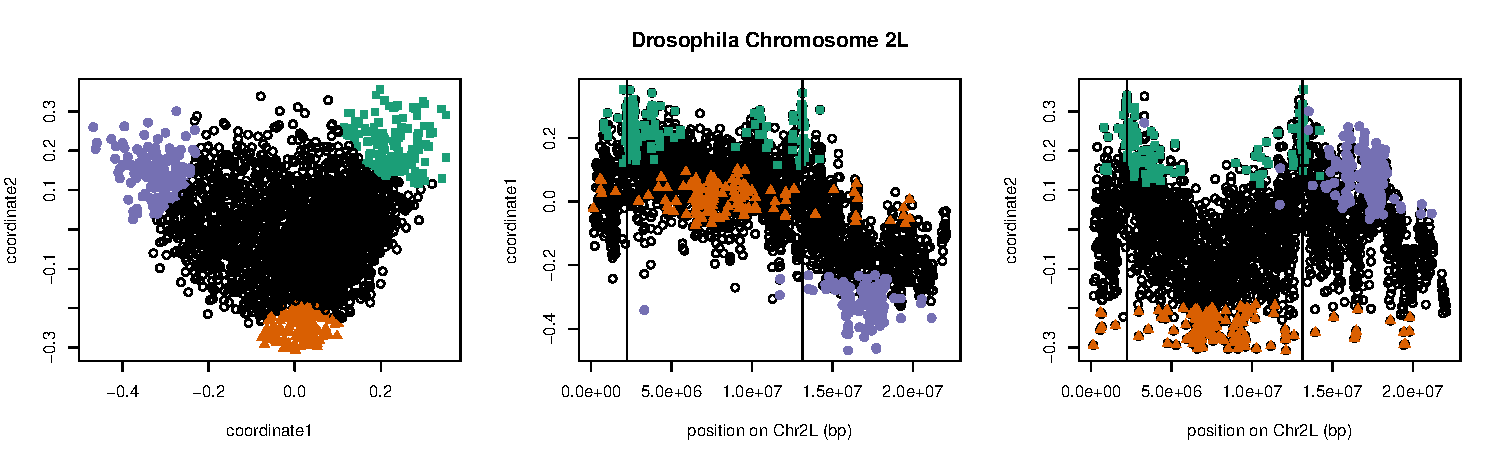
\includegraphics[width=0.9\textwidth]{Fig1_Together_MDS_plot_Chr2L_final_abline}
    \end{center}
    \caption{
         Variation in structure for windows on chromosome arm Chr2L. 
         Each represents a window: (a) shows the MDS visualization of relationships between windows. 
         (b) and (c) show the position (midpoint) of each window against the first and second MDS coordinates, respectively. 
         Colors are consistent for (a) (b) and (c).
         Vertical black lines show the breakpoints of known polymorphic inversions In(2L)t.
         \label{fig:mds_chr2L}
    }
\end{figure}


We pick a window for each extreme, and take out 5\% windows that are closest to it in the MDS 2D plot , then combine those windows for each extreme and apply PCA on them. (Figure \ref{fig:pca_chr2L}) We can see the obvious difference between their PCA plots. This difference stands for variation of population structure along the genome in \textit{Drosophila} Chr2L.

\begin{figure}
    \begin{center}
       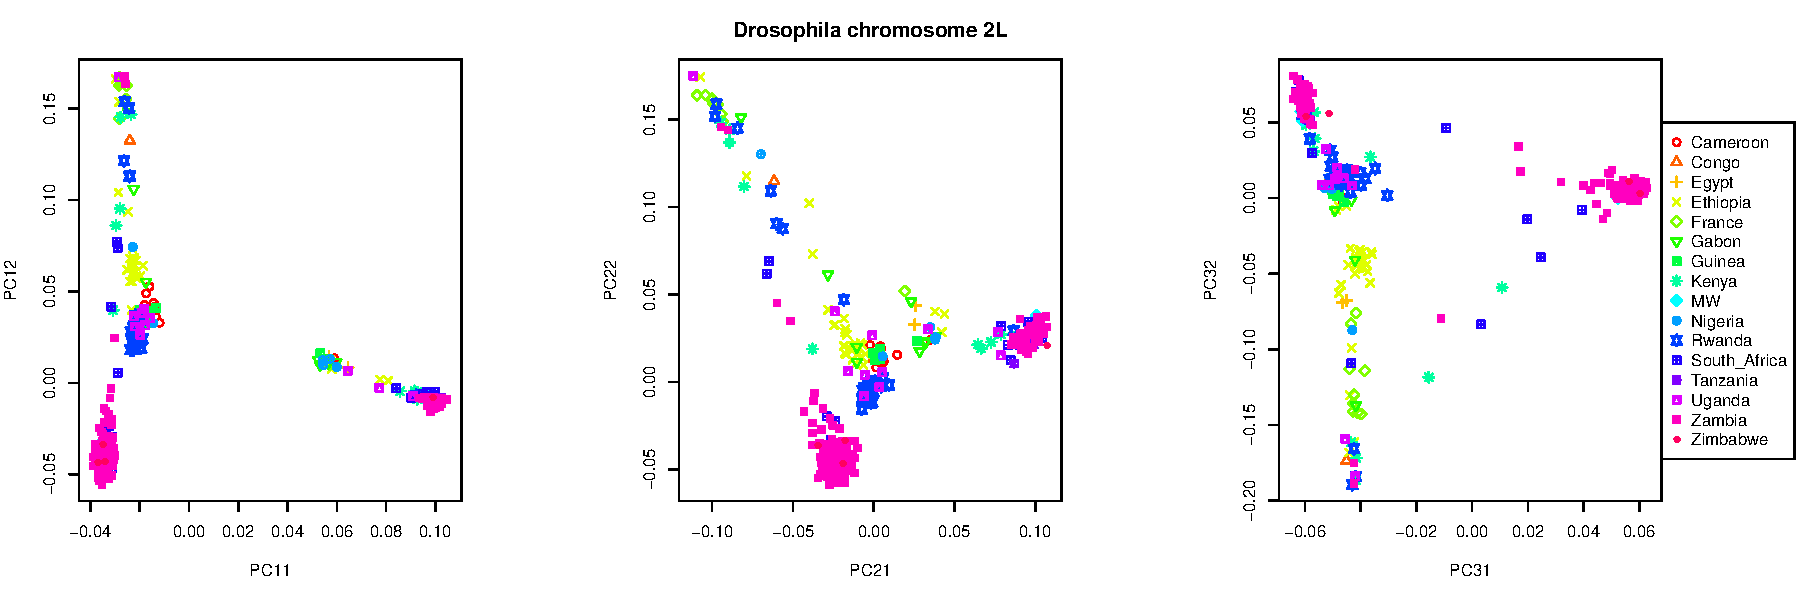
\includegraphics[width=0.9\textwidth]{Fig2_all_pca_plots_for_Chr2L_3peaks_byMDS}
    \end{center}
    \caption{
        PCA plots for each peak in Figure \ref{fig:mds_chr2L}a. 
        Each point represents a sample. 
        The plots are plotting the second principal components against the first principal components. 
        (a) shows the windows colored green in Figure 1; 
        (b) shows orange windows; and (c) shows purple windows.
         \label{fig:pca_chr2L}
    }
\end{figure}


There's a known inversion in Chr2L in \textit{Drosophila}, In(2L)t, with breakpoints at 2225744bp and 13154180bp. \citep{corbett2012population} We recolored the PCA plots in Figure \ref{fig:pca_chr2L} a,b,c by the direction of the inversion for each sample using data from John Pool's lab \citep{lack2015drosophila}. Figure \ref{fig:color_inver}
\plr{(citation?)}
The results show that PCA plots, and thus population structure, varies significantly along the genome, with most variation closely related to inversions. 
Extremes of structure occurred around inversion breakpoints or in the centers of inversions (green and orange parts in Chr2L).
The corresponding PCA plots show that locally, population structure is mostly determined by which orientation of the inversion each sample has.
Similar results are found in other chromosome arms that have known polymorphic inversions (Chr2R, Chr3L, Chr3R) in \textit{Drosophila}. (See supplementary for more details)
These facts show that the variation of population structure along the Drosophila genome is mainly due to inversions.

\begin{figure}
    \begin{center}
       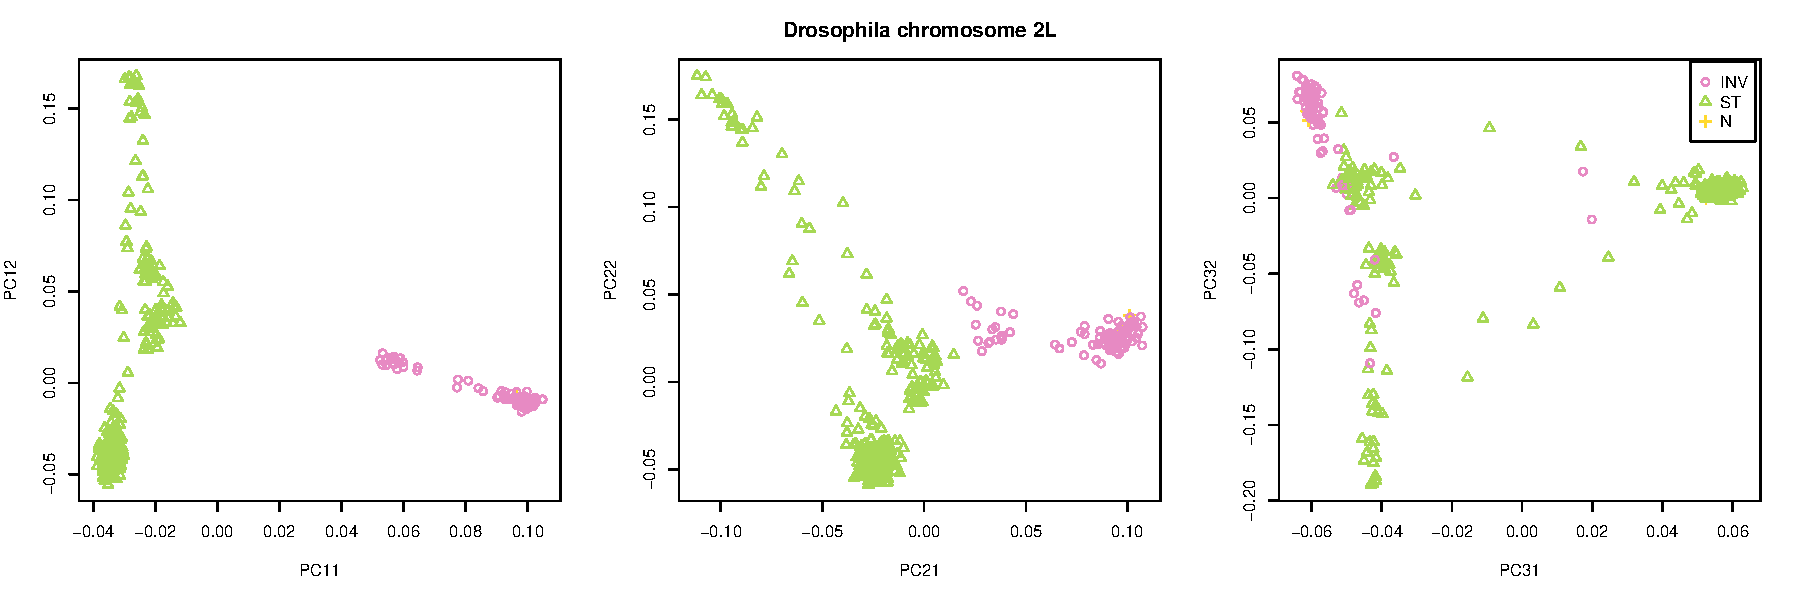
\includegraphics[width=0.9\textwidth]{Fig3_all_pca_plots_for_Chr2L_3peaks_color_by_In2Lt_byMDS}
    \end{center}
    \caption{
         As in Figure 2, except that samples are colored by orientation of the corresponding polymorphic inversion, In(2L)t.
        \label{fig:color_inver}
    }
\end{figure}

\subsection{Human}
We ran our method separately on all 22 autosomes. 
We found that the windows that are outliers in the first MDS coordinate (Figure \ref{fig:mds_human}b) coincide with the position of known polymorphic inversions on 8p23. 
Similar results are found in other chromosomes that have known polymorphic inversions (Chromosome 15, Chromosome 17) in Human. (See supplementary for more details)
Similar to Drosophila, the biggest source of variability in population structure along each human chromosome seems to be polymorphic inversions. Other chromosomes showed similar results around predicted inversions: PCA might provide an additional way to identify inversions \citep{ma2012investigation}.
When we run the process for all 22 autosomes together, the outlying signal of chromosome 8 is still impressing. (See supplementary for all 22 autosomes' MDS results for human)

\plr{Readers will wonder if the "triangle" looks the same in humans and Medicago as in Drosophila. Should we add them, or just put these in the supplement?}

\plr{Do we know what happens when we run all 22 autosomes together?}

\begin{figure}
    \begin{center}
       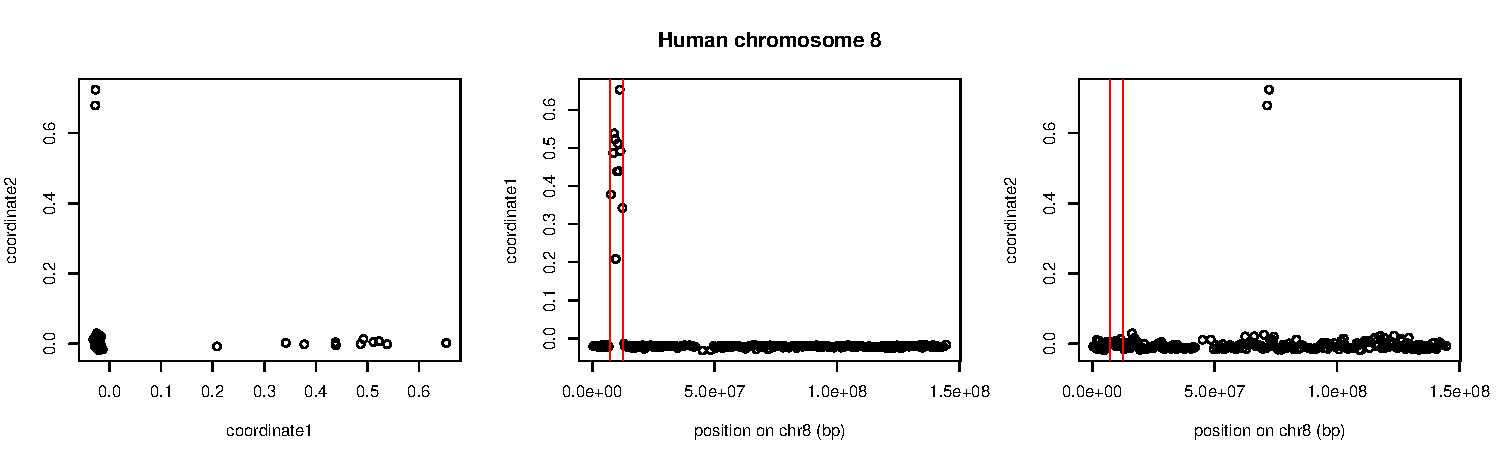
\includegraphics[width=0.7\textwidth]{Fig4_POPRES_Together_MDS_plot_chr8_final_abline}
    \end{center}
    \caption{
         Variation in structure between windows on human chromosome 8. Each point in the plot represents a window. 
         (a) shows the MDS visualization of relationships between windows; 
         (b) and third (c) show the two MDS coordinates of each window against its position (midpoint) along the chromosome. 
         The vertical red lines show the breakpoints of the known inversion on 8p23. \citep{antonacci2009characterization}
        \label{fig:mds_human}
    }
\end{figure}


\subsection{\textit{Medicago truncatula}}
We checked the MDS results for all 8 chromosomes. 
\plr{The results looked different than the other two species, with much less pronounced peaks...}
We found the position of the peak for each MDS plot has a coincidence with the position of heterochromatic regions. This means the population structure in the windows located in heterochromatin tends to have higher similarity, since those windows are closer in MDS plots. (Figure \ref{fig:mds_medicago}) Biologically,
heterochromatic regions have lower gene density and may be less subject to selection \citep{kulikova2001integration,paape2013selection}. Then we checked the MDS results against gene density along the genome for each chromosome using gene models in Mt4.0 JBrowse. Numerically, the first MDS coordinate value is negatively correlated to the gene count for each window, which shows the correlation between MDS result and gene density. (Figure \ref{fig:mds_gene_count}) 
This fact shows that in \textit{Medicago truncatula}, variation in population structure, as measured by the first MDS coordinate, is negatively correlated to gene density. 
Unlike in the human and Drosophila genomes, in \textit{Medicago truncatula}, major variation in population structure is likely due to linked selection. 

\begin{figure}
    \begin{center}
       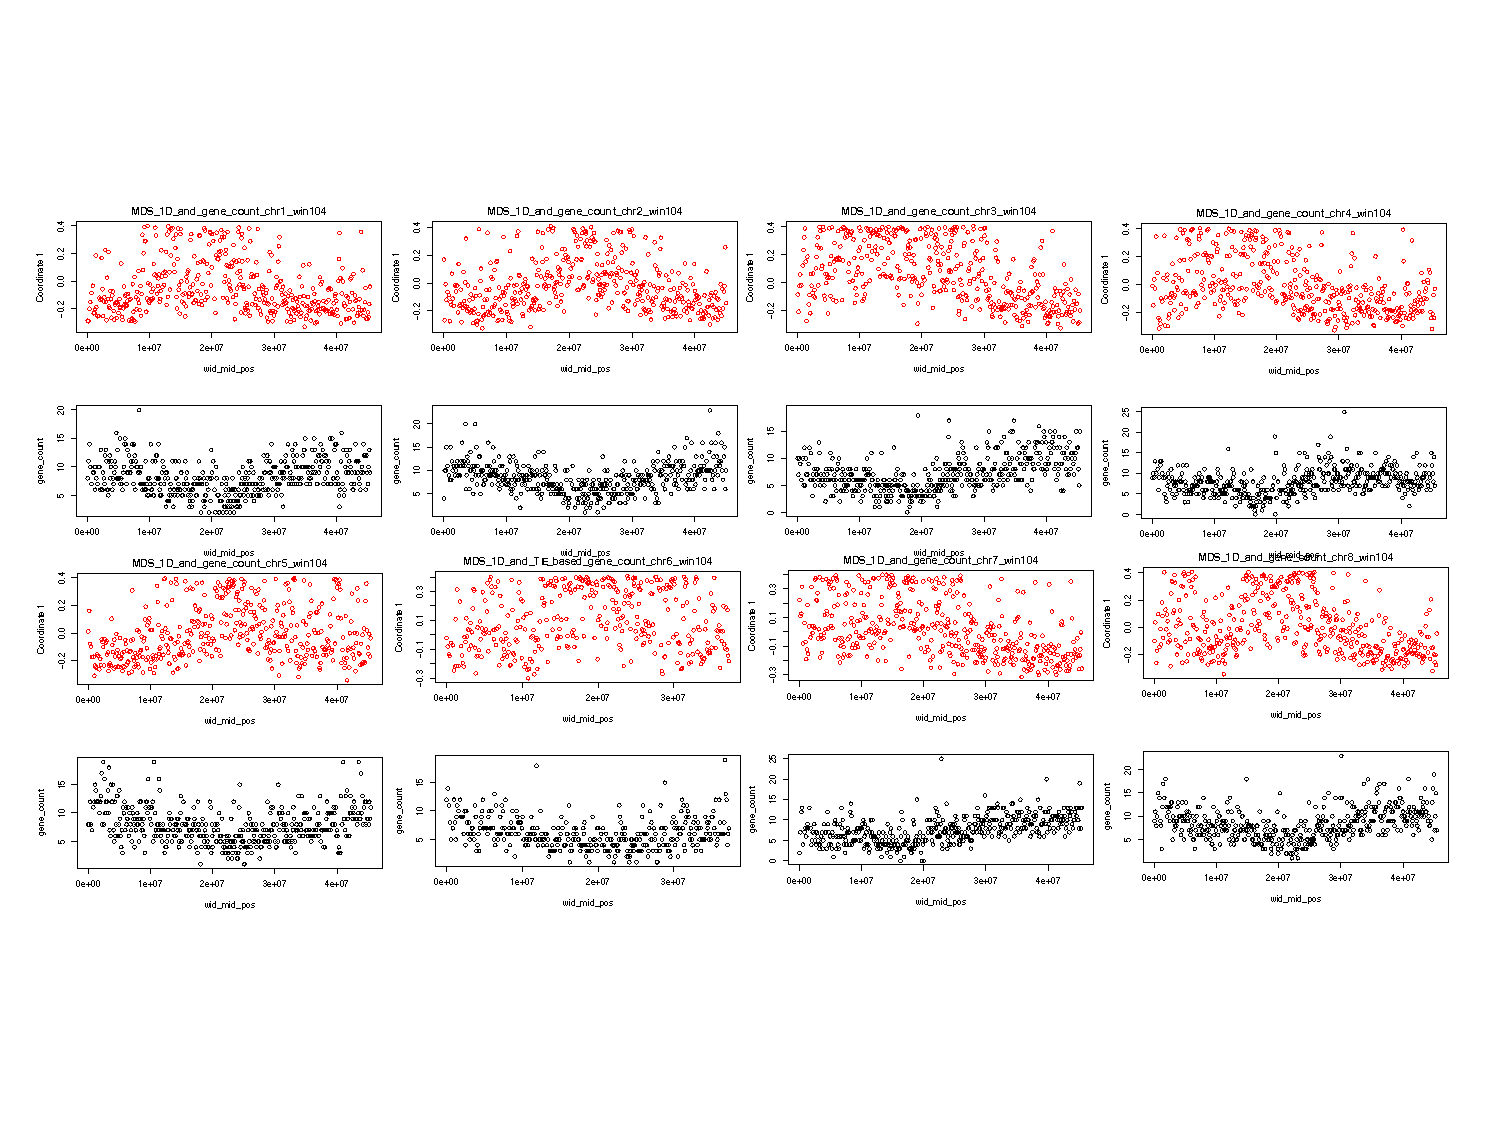
\includegraphics[width=0.7\textwidth]{fig5}
    \end{center}
    \caption{
         MDS results for the \textit{Medicago} genome (chr1-8), using first coordinate of MDS against the middle position of each window along each chromosome. 
         The bars under MDS plots are diagrams for each chromosome showing the relative position of heterochromatin (the deep purple part on each bar) \citep{kulikova2004satellite, kulikova2001integration}.
        \label{fig:mds_medicago}
    }
\end{figure}


\begin{figure}
    \begin{center}
       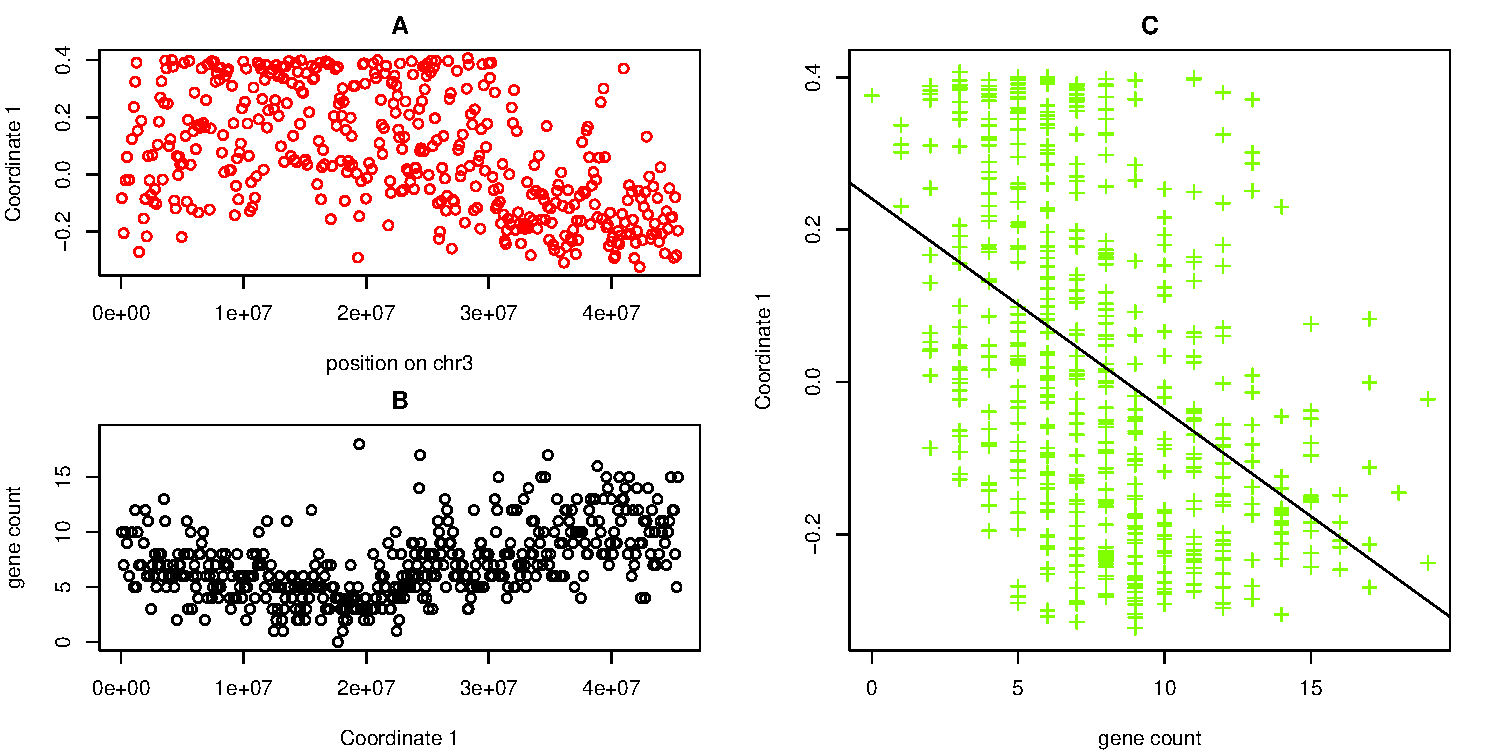
\includegraphics[width=0.9\textwidth]{Fig6_MDS_1D_and_gene_count_and_lm_chr3_based_all_chr_win104}
    \end{center}
    \caption{
        First MDS coordinate against gene density for chromosome 3. 
        (A) First MDS coordinate against the position (midpoint) of each window. 
        (B) Gene count for each window against the position of each window; 
        (C) The first MDS coordinate is significantly correlated with gene count (r=XXX, p=XXX). 
        (See supplementary for other chromosomes' MDS results against gene count for \textit{Medicago})
        \label{fig:mds_gene_count}
    }
\end{figure}

%%%%%%% %%%%%%%%%
\section{Discussion}

We've shown that local summaries of tree shape, i.e., kinship, vary significantly on a large scale along the genome,
and that exploratory visualization of this variation can be useful.

There are many ways to visualize population structure; perhaps others would show different things.

Come back to some points in the Introduction.

\subsection{Future work}
1. For human and Drosophila, we want to eliminate the regions under known inversions and check the variation of population structure for the remaining part by removing those sections. We try to check whether they will give similar results as in \textit{Medicago truncatula}, that is whether the variation is closely related to heterochromatin or gene density.

\noindent 2. Uneven sampling has a strong influence on PCA projections \citep{mcvean2009genealogical}. 
Our human data, POPRES, is unevenly sampled including 346 African-Americas, 73 Asians, 359 Indian Asians and 3187 Europeans. 
First, we'll try sub-sampling Europeans to balance the population size for the 4 population and repeat the process on the resampled data. 
Second, we'll try to apply the whole process on only European samples to see the genetic variation inside European samples. 
Third, we want to try different scheme of adding a weighting matrix to the covariance matrix of genotype data, thus to the reduce the influence of uneven sampling.

\noindent 3. Since regions that have low recombination rate tend to have similar PCs, we'll try cutting the chromosomes into windows with same distance in genetic map instead of same SNP numbers.

\noindent 4. Euclidean distance between the contracted matrix based on PCs is one measure of the similarity for window's population structure.
We want to try other methods of distance between windows, for example, we used the distance for PCs to reduce noise, however the distance between covariance matrixes of genotype matrix might also be informative.

\noindent 5. Although the first two coordinates contains the main part of information, we'd like to see the information contained in higher PCs (e.g. the third PC, the forth PC), and higher dimension of MDS.

\bibliographystyle{plainnat}
\bibliography{references}  
\end{document}  
